% !TeX program = lualatex
\documentclass[tikz,border=6pt]{standalone}

\usepackage{tikz}
\usetikzlibrary{calc,angles,quotes}

\begin{document}
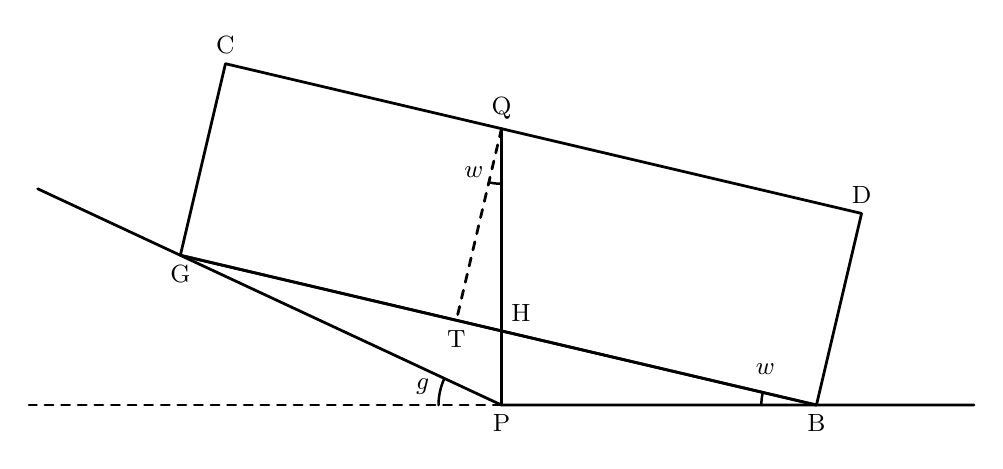
\begin{tikzpicture}[x=1cm,y=1cm, line cap=round, line join=round, font=\small]

% =========================
% 1) THAM SỐ HÓA (đổi ở đây)
% =========================
\def\alpha{25}   % góc dốc của mặt đường (độ)
\def\Lext{6}     % độ dài phần đường ngang (từ P sang phải)
\def\Lback{6.5}  % độ dài kéo dài đường dốc về bên trái (từ P)
\def\b{4}        % tọa độ x của B (B nằm trên mặt đường ngang y=0)
\def\tG{4.5}     % khoảng cách từ P đi lên-trái trên dốc để tới G
\def\h{2.5}      % chiều cao thùng xe (vuông góc với GB)

% =========================
% 2) TIỀN TÍNH TOÁN (tránh lỗi calc)
% =========================
\pgfmathsetmacro{\dxBack}{-\Lback*cos(\alpha)}
\pgfmathsetmacro{\dyBack}{ \Lback*sin(\alpha)}

\pgfmathsetmacro{\Gx}{-\tG*cos(\alpha)}
\pgfmathsetmacro{\Gy}{ \tG*sin(\alpha)}

\pgfmathsetmacro{\dxPleft}{-1.2*cos(\alpha)}
\pgfmathsetmacro{\dyPleft}{ 1.2*sin(\alpha)}

% =========================
% 3) ĐIỂM MỐC: P là gốc
% =========================
\coordinate (P) at (0,0);
\coordinate (G) at (\Gx,\Gy);
\coordinate (B) at (\b,0);

% =========================
% 4) DỰNG HÌNH CHỮ NHẬT G-C-D-B
% =========================
% véc-tơ w = B - G
\pgfmathsetmacro{\wx}{\b - \Gx}
\pgfmathsetmacro{\wy}{0 - \Gy}
\pgfmathsetmacro{\Lw}{sqrt(\wx*\wx+\wy*\wy)}

% pháp tuyến đơn vị n = (-wy, wx)/|w|
\pgfmathsetmacro{\nx}{-(\wy)/\Lw}
\pgfmathsetmacro{\ny}{ (\wx)/\Lw}

% C = G + h n,  D = B + h n
\pgfmathsetmacro{\Cx}{\Gx + \h*\nx}
\pgfmathsetmacro{\Cy}{\Gy + \h*\ny}
\pgfmathsetmacro{\Dx}{\b  + \h*\nx}
\pgfmathsetmacro{\Dy}{0   + \h*\ny}
\coordinate (C) at (\Cx,\Cy);
\coordinate (D) at (\Dx,\Dy);

% =========================
% 5) Q là giao của CD với đường thẳng đứng x=0
% =========================
\pgfmathsetmacro{\tQ}{(0-\Cx)/(\Dx-\Cx)}
\pgfmathsetmacro{\Qx}{\Cx + \tQ*(\Dx-\Cx)}
\pgfmathsetmacro{\Qy}{\Cy + \tQ*(\Dy-\Cy)}
\coordinate (Q) at (\Qx,\Qy);

% =========================
% 6) H là giao của GB với x=0
% =========================
\pgfmathsetmacro{\tH}{(0-\Gx)/(\b-\Gx)}
\pgfmathsetmacro{\Hx}{\Gx + \tH*(\b-\Gx)}
\pgfmathsetmacro{\Hy}{\Gy + \tH*(0-\Gy)}
\coordinate (H) at (\Hx,\Hy);

% ============================================================
% 6bis) Tính góc w = ∠GBP (độ) và dựng T sao cho ∠TQH = w
% ============================================================
% Hướng tia BG và tia BP
\pgfmathsetmacro{\angBG}{atan2(\Gy-0, \Gx-\b)} % hướng từ B đến G
\pgfmathsetmacro{\wDeg}{abs(180-\angBG)}       % vì hướng BP là 180°

% Dựng tia từ Q sao cho tạo với QH (hướng xuống) một góc w về phía trái:
% hướng xuống là -90°, nên hướng QT = -90° - w
\pgfmathsetmacro{\thetaQT}{-90-\wDeg}
\pgfmathsetmacro{\ux}{cos(\thetaQT)}
\pgfmathsetmacro{\uy}{sin(\thetaQT)}

% Giao điểm T của đường thẳng: Q + t*u với đường thẳng GH: G + s*(H-G)
\pgfmathsetmacro{\vx}{\Hx-\Gx}
\pgfmathsetmacro{\vy}{\Hy-\Gy}
\pgfmathsetmacro{\dx}{\Qx-\Gx}
\pgfmathsetmacro{\dy}{\Qy-\Gy}
\pgfmathsetmacro{\det}{\vx*\uy-\vy*\ux}

% s = det((Q-G), u) / det(v, u)
\pgfmathsetmacro{\sT}{(\dx*\uy-\dy*\ux)/\det}
\pgfmathsetmacro{\Tx}{\Gx+\sT*\vx}
\pgfmathsetmacro{\Ty}{\Gy+\sT*\vy}
\coordinate (T) at (\Tx,\Ty);

% =========================
% 7) VẼ THEO KHỐI
% =========================
% Mặt đường: dốc + ngang
\draw[line width=1.0pt] ($(P)+(\dxBack,\dyBack)$) -- (P) -- ($(P)+(\Lext,0)$);

% Mặt đường: kéo trái (nét đứt)
\draw[dashed, line width=1.0pt] (P) -- ($(P)-(\Lext,0)$);

% Thùng xe
\draw[line width=1.0pt] (G) -- (C) -- (D) -- (B) -- cycle;

% Đường chéo GB
\draw[line width=1.0pt] (G) -- (B);

% Đường thẳng đứng qua Q xuống P
\draw[line width=1.0pt] (Q) -- (P);

% Thêm tia QT để thể hiện góc TQH
\draw[dashed, line width=1.0pt] (Q) -- (T);

% PK (nét đứt như hình mẫu ở trang trước; ở hình này là QP nét đứt? bạn có thể bỏ nếu không cần)
% (giữ nguyên: không thêm PK ở đây)

% =========================
% 8) KÝ HIỆU / NHÃN
% =========================
% Góc alpha tại P
% \coordinate (Pright) at ($(P)+(1.2,0)$);
% \coordinate (Pleft)  at ($(P)+(\dxPleft,\dyPleft)$);
% \draw pic[draw, angle radius=0.65, angle eccentricity=1.25] {angle = Pright--P--Pleft};

% Nhãn điểm
\node[above] at (C) {C};
\node[above] at (D) {D};
\node[below] at (G) {G};
\node[below] at (B) {B};
\node[above] at (Q) {Q};
\node[above right] at (H) {H};
\node[below] at (P) {P};
\node[below] at (T) {T};

% Góc g giữa dốc và mặt đường
\coordinate (Xroad) at ($(P)-(1,0)$);
\coordinate (Xslope) at ($(P)+(-1,{tan(\alpha)})$);
\pic[draw, line width=0.9pt, angle radius=8mm]
  {angle=Xslope--P--Xroad};
\node at ($(P)+(-1,{tan(\alpha)/2})$) {$g$};

% ------------------------------------------------------
% (1) Ghi chú góc GBP = w tại B
% góc giữa BG và BP (BP hướng về P)
\pic[draw, line width=0.9pt, angle radius=7mm]
  {angle=G--B--P};
\node at ($(B)+(-0.65,0.45)$) {$w$};

% (2) Trên GH có T sao cho ∠TQH = w, vẽ góc tại Q
\pic[draw, line width=0.9pt, angle radius=7mm]
  {angle=T--Q--H};
\node at ($(Q)+(-0.35,-0.55)$) {$w$};

\end{tikzpicture}
\end{document}
